
	Creamos un set de datos en el cual pudiésemos esperar valores conocidos. Además acotamos a un diccionario de solo tres elementos, el Accurracy obtenido es:
	
	
	
	\begin{figure}[h] 
		\centering
			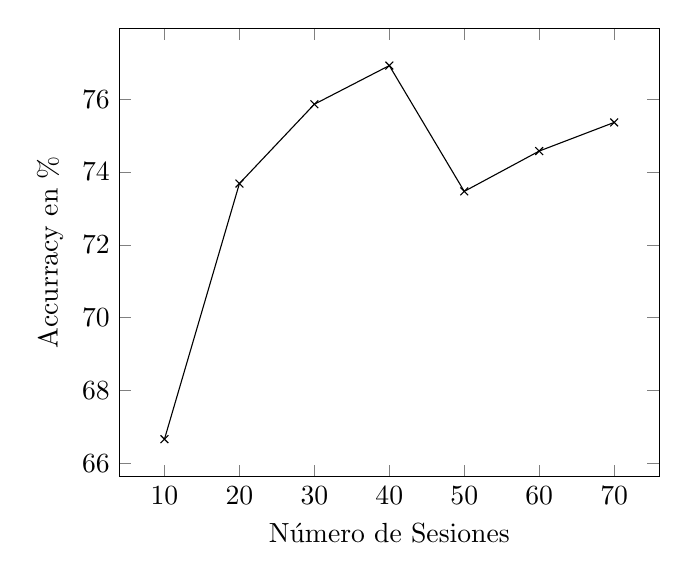
\begin{tikzpicture}
			\begin{axis}[
			xlabel= Número de Sesiones,
			ylabel=Accurracy en \% ]
			\addplot[color=black,mark=x] coordinates {
				(10, 66.6666666666666)
				(20, 73.6842105263157)
				(30, 75.8620689655172)
				(40, 76.9230769230769)
				(50, 73.469387755102)
				(60, 74.5762711864406)
				(70, 75.3623188405797)
			};
			\end{axis}
			\end{tikzpicture}	
		\caption{Experimento con set de datos sintéticos.}
		\label{fig:graph-exp1}
	\end{figure}
	

	
 
	
	En el gráfico \ref{fig:graph-exp1} usamos como mínimo 10 sesiones de las 80 de disponibles que se usaron par este experimento. Dado a que en este caso la cantidad de sesiones es bien reducida y cada símbolo posee una gran frecuencia existe mayor redundancia de datos y nuestro modelo se comporta como espera que lo haga un algoritmo de compresión de datos. Entre mayor es la cantidad de símbolos iguales
	que van entrenando al \emph{trie}, hay una aglomeración de frecuencia en ciertos nodos, pero estos son minimizados por los niveles que genera al momento de la construcción del árbol.
	
	La tasa de frecuencia de un símbolo converge a predicciones de secuencias evaluadas que caen en el nodo con mejor probabilidad dado $\epsilon$ (raíz del \emph{trie}).
	



	
   \begin{figure}[h] 
	   \centering
	   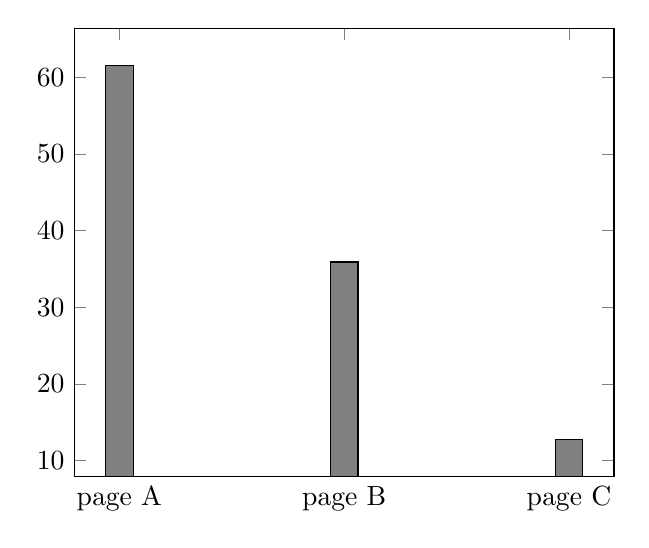
\begin{tikzpicture}
	   \begin{axis}[
	   symbolic x coords={ page A, page B, page C},
	   xtick=data
	   ]
	   \addplot[ybar,fill=gray] coordinates {
	   	(page A,   61.5)
	   	(page B,  35.9)
	   	(page C,   12.8)
	   };
	   \end{axis}
	   \end{tikzpicture}
		\caption{Distribución de símbolos para set de datos sintéticos.}
		\label{fig:bar-chart-data-sintetica}
	\end{figure}


	\begin{table}[]
		\centering
		\label{tabla-exp-1}
		\begin{tabular}{ccccc}
			\textbf{pruebas}     & \textbf{entrenamiento} & \textbf{accuracy}    & \textbf{nodos}       & \textbf{niveles}     \\
			10                   & 90                     & 0,753623188405797    & 10                   & 5                    \\
			20                   & 80                     & 0,745762711864406    & 10                   & 5                    \\
			30                   & 70                     & 0,73469387755102     & 10                   & 5                    \\
			40                   & 60                     & 0,769230769230769    & 10                   & 5                    \\
			50                   & 50                     & 0,758620689655172    & 10                   & 5                    \\
			60                   & 40                     & 0,736842105263157    & 10                   & 5                    \\
			70                   & 30                     & 0,666666666666666    & 10                   & 5                    \\
			&                        &                      &                      &                      \\
			\multicolumn{1}{l}{} & \multicolumn{1}{l}{}   & \multicolumn{1}{l}{} & \multicolumn{1}{l}{} & \multicolumn{1}{l}{}
		\end{tabular}
		\caption{ Resumen de datos experimento 1}
	\end{table}






	\begin{table}[] 	\label{tabl-exp-1-frec}
		\centering
		\resizebox{0.9\textwidth}{!}{% <------ Don't forget this %
	
		\begin{tabular}{lccccccccccccccccc}
			\textbf{símbolo}    & A  & B  & C  & D  & E & F  & G  & H  & I  & J  & K & L  & M  & N  & O & P & Q \\
			\textbf{frecuencia} & 400 & 280 & 100 & 0 & 0 & 0 & 0 & 0 & 0 & 0 & 0 & 0 & 0 & 0 & 0 & 0 & 0
		\end{tabular}
		
	}
		\caption{Tabla de frecuencia experimento 1}
	\end{table}



	Tal como se puede ver en el gráfico \ref{fig:bar-chart-data-sintetica} existe un gran probabilidad de que dado una secuencia de accesos después de $\epsilon$ la próxima sección a acceder sea la página A.
	Esto es adicionalmente es consistente a el tipo de set de datos que hemos ocupado ya que con esto podemos delimitar a que nuestro modelo al tener símbolos bastante frecuente no crea un trie desbalanceado, para este caso solo acota constantemente a un altura de 5 niveles y una variación mínima entre la exactitud, que posee el entrenamiento versus set de evaluaciones, incluso podemos solo podemos usar un entrenamiento de por lo menos 30 sesiones para predecir 50 sesiones con un Accurracy con un margen de error máximo de $10\%$ en el peor de los casos. 
	Lo anterior si lo comparamos con un evento aleatorio como resultado nos daría que nuestro modelo es bastante mejor que una predicción aleatoria, es decir $ 66.7\%  \geq 33\%$, siendo esta una comparativa optimista de que al menos nuestro modelo dado un set de datos artificial.
	



	